
\begin{frame}
 \frametitle{Tracking}
\begin{enumerate}
\item
Build distance matrix $\vec{D}(old,new)$ between all eddies($t=now-dt$) to all eddies($t=now$).
\item
Flag all $\vec{D}(old,new) > $ threshld.
\item
Flag all not meeting a \textit{similarity criterion} (function of scale and amplitude).
\item
$min(\vec{D})$ in both directions.
\begin{itemize}
\item
agreement: eddy is tracked!\\
$\rightarrow$ append to respective track in running archive.
\item
no new eddy agrees with old eddy: eddy just died..\\
$\rightarrow$ if age $\ge$ threshold, write track to archive, else delete!
\item
no old eddy agrees with new eddy: a new eddy was born\\
$\rightarrow$ initiate new track in running archive.
\end{itemize}
\end{enumerate}
\end{frame}


\begin{frame}[noframenumbering]
 \frametitle{Tracking}
\begin{enumerate}
\item
Build distance matrix $\vec{D}(old,new)$ between all eddies($t=now-dt$) to all eddies($t=now$).
\item
Flag all $\vec{D}(old,new) > $ threshld.
\item
Flag all not meeting a \textbf{\textit{similarity criterion}} (\textbf{function of scale and amplitude}).
\item
$min(\vec{D})$ in both directions.
\begin{itemize}
\item
agreement: eddy is tracked!\\
$\rightarrow$ append to respective track in running archive.
\item
no new eddy agrees with old eddy: eddy just died..\\
$\rightarrow$ if age $\ge$ threshold, write track to archive, else delete!
\item
no old eddy agrees with new eddy: a new eddy was born\\
$\rightarrow$ initiate new track in running archive.
\end{itemize}
\end{enumerate}
\end{frame}


\begin{frame}
\frametitle{What is the scale and amplitude of an eddy ???}
 \begin{figure}
\centering
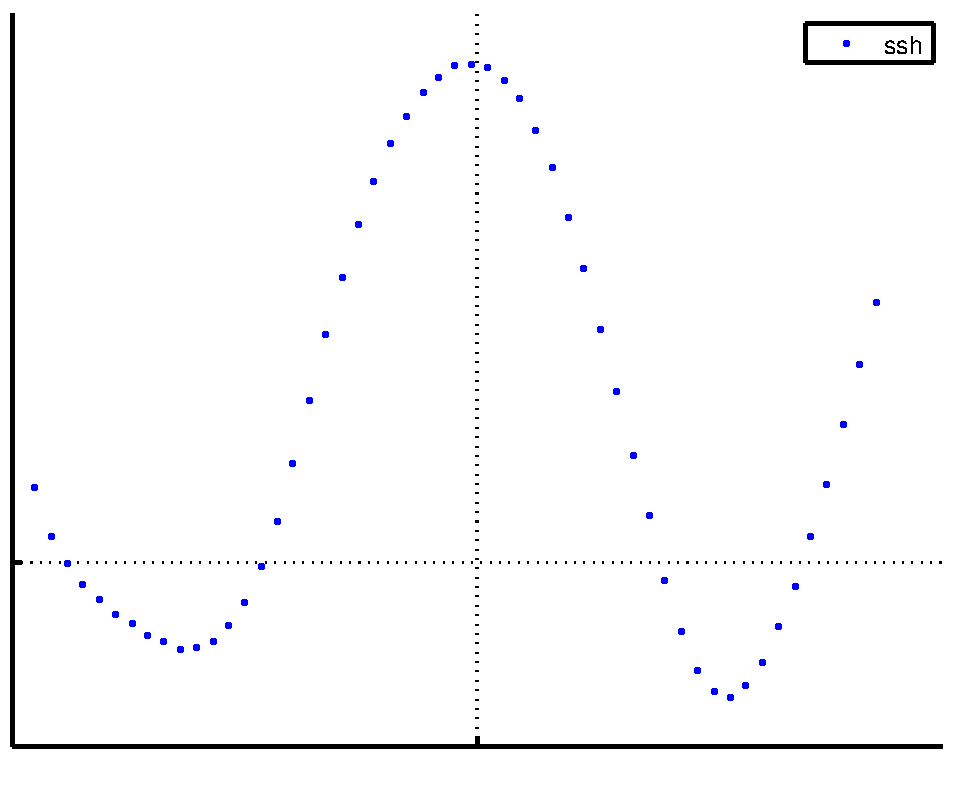
\includegraphics[height=200pt,keepaspectratio=true]{Na.pdf}
\end{figure}
\end{frame}


\begin{frame}
 \frametitle{example: meander}
\begin{figure}
\centering
	%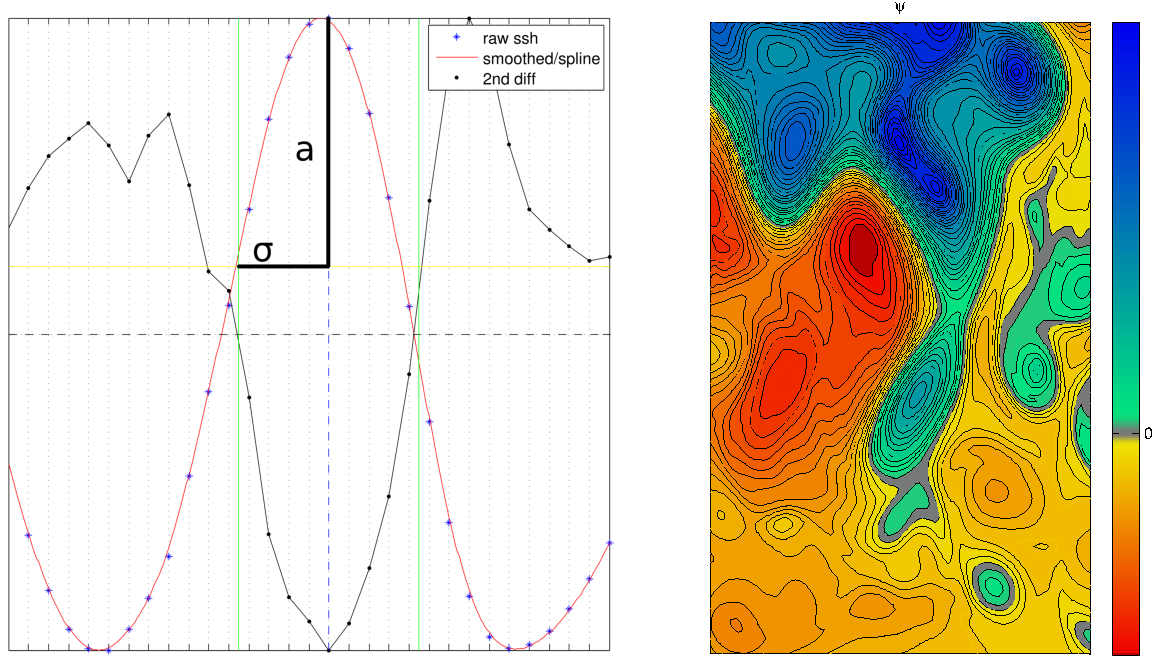
\includegraphics[width=300pt,keepaspectratio=true]{prof3bPsi.pdf}
	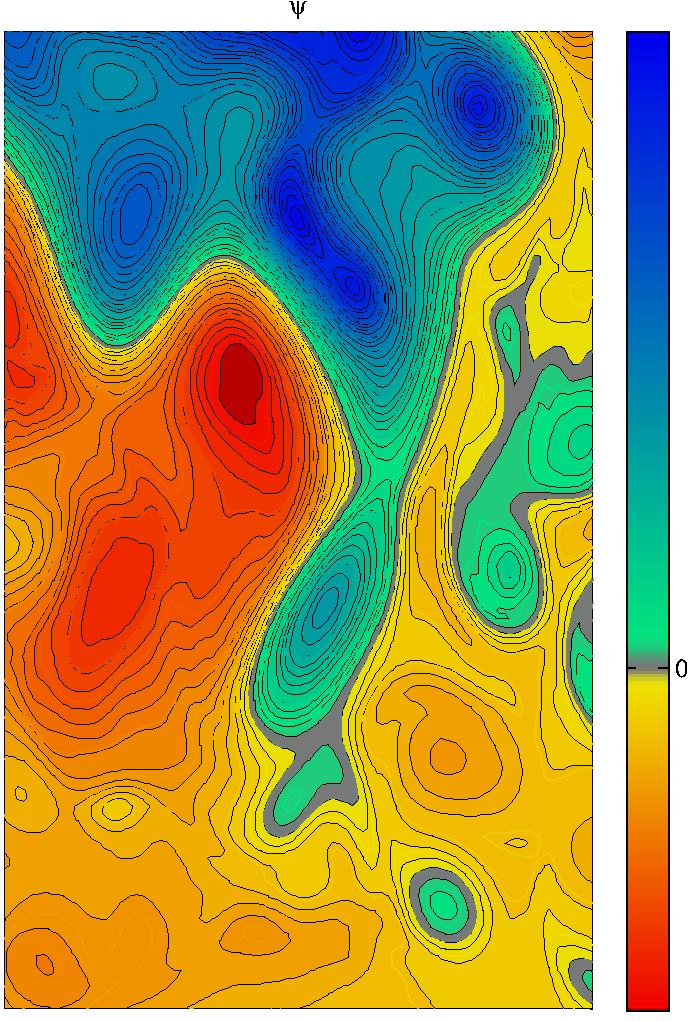
\includegraphics[height=200pt,keepaspectratio=true]{psi.pdf}
\end{figure}
\end{frame}


\begin{frame}
\frametitle{Problem: coarse resolution}
$ \partial_x \sim \vec{U}, \; \partial_{xx} \sim \vec{\omega}$
 \begin{figure}
\centering
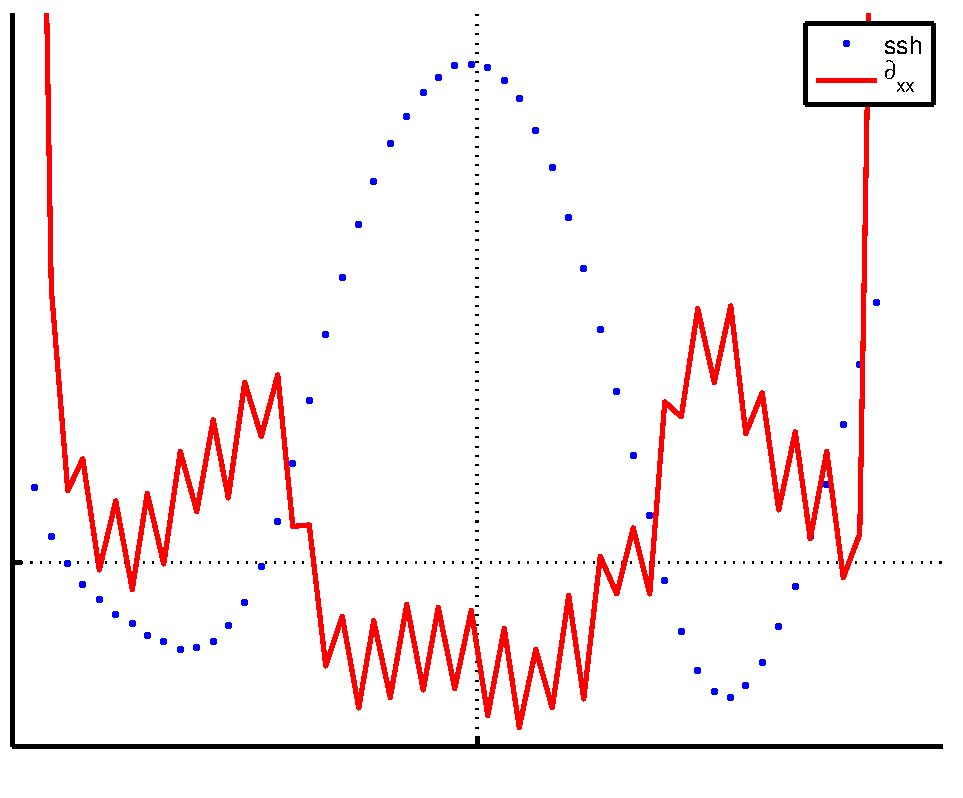
\includegraphics[height=200pt,keepaspectratio=true]{Nb.pdf}
\end{figure}
\end{frame}


\begin{frame}
\frametitle{Solution: Interpolate and use Fourier Series for differentials}
 \begin{figure}
\centering
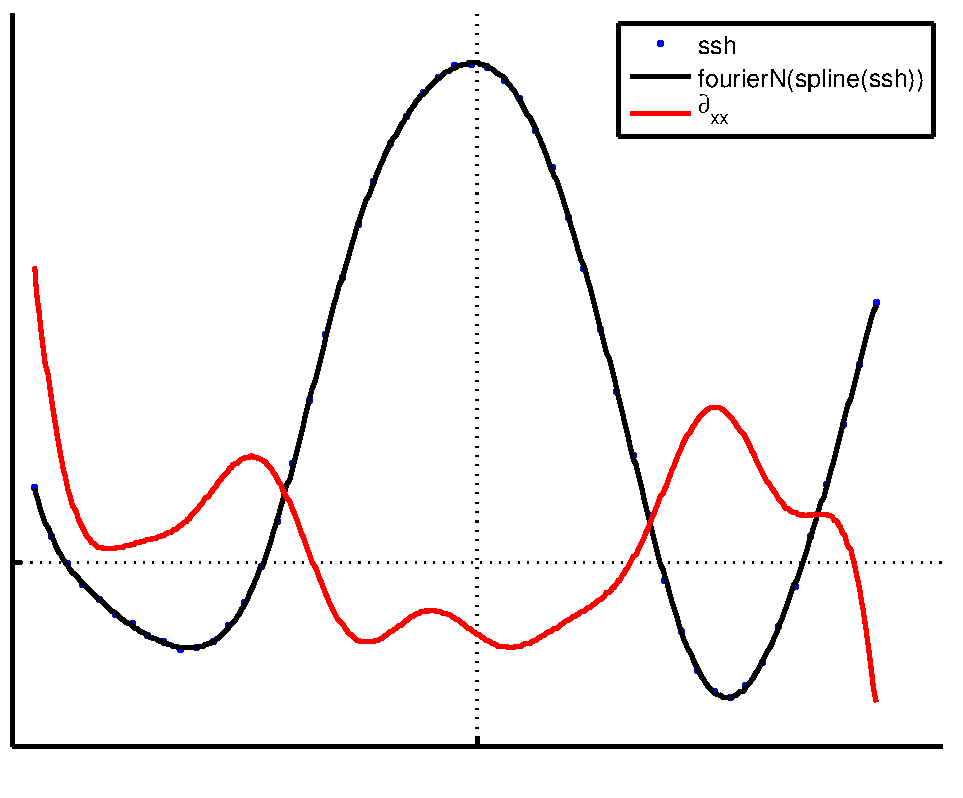
\includegraphics[height=200pt,keepaspectratio=true]{Nc.pdf}
\end{figure}
\end{frame}

\begin{frame}
\frametitle{Assuming gauss shape:  $A \exp{\left(- x^2/2\sigma^2\right)}; \;\;a=A(1-\exp{-1/2})$}
All shape-defining parameters for the \textit{similarity criterion} are determined!  
 \begin{figure}
\centering
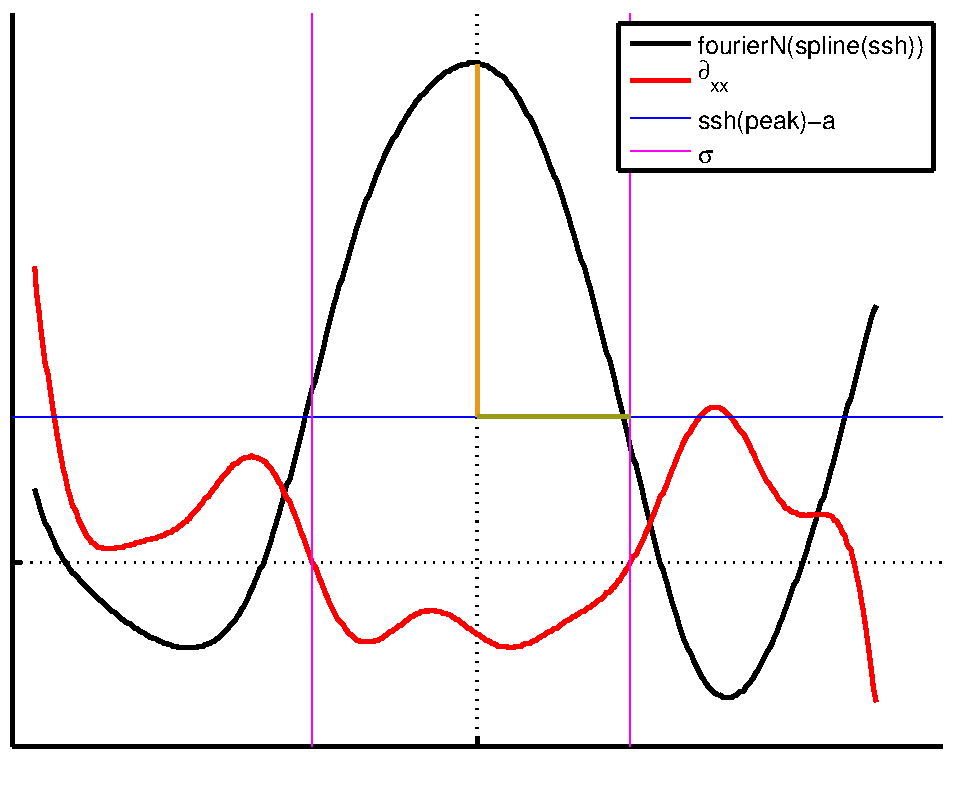
\includegraphics[height=200pt,keepaspectratio=true]{Ne.pdf}
\end{figure}
\end{frame}


\begin{frame}
\frametitle{Note: Gauss shape assumption not necessary for this method.}
 \begin{figure}
\centering
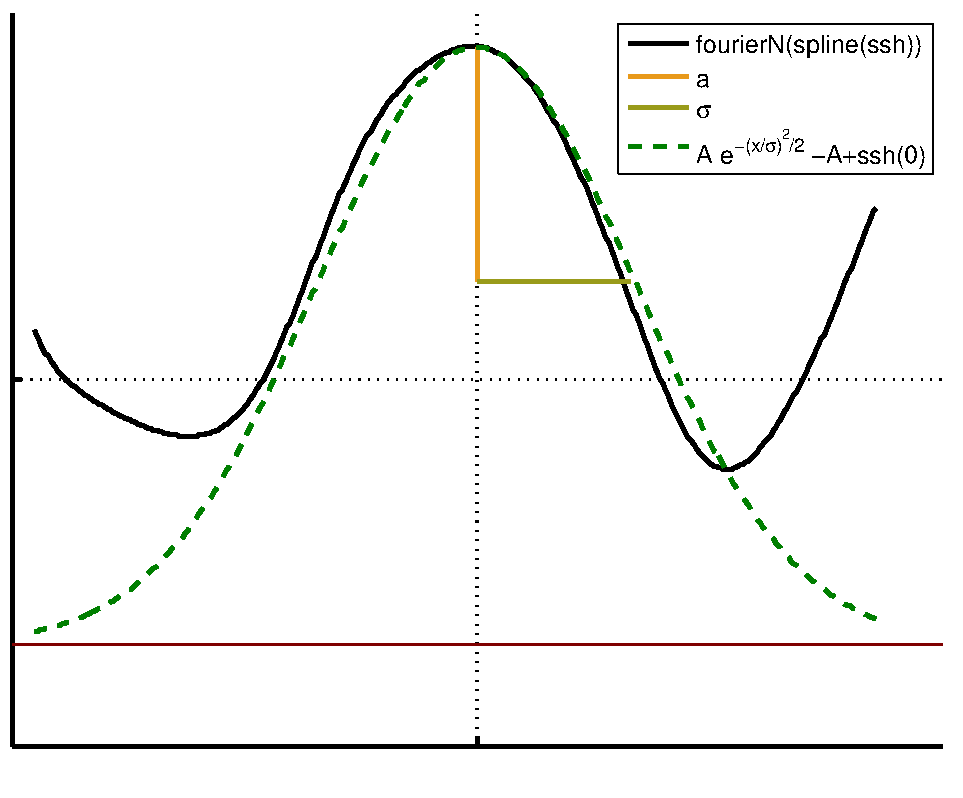
\includegraphics[height=200pt,keepaspectratio=true]{Nf.pdf}
\end{figure}
\end{frame}

\begin{frame}
\frametitle{Chelton et al. define 4 different eddy scales.}
 \begin{figure}
\centering
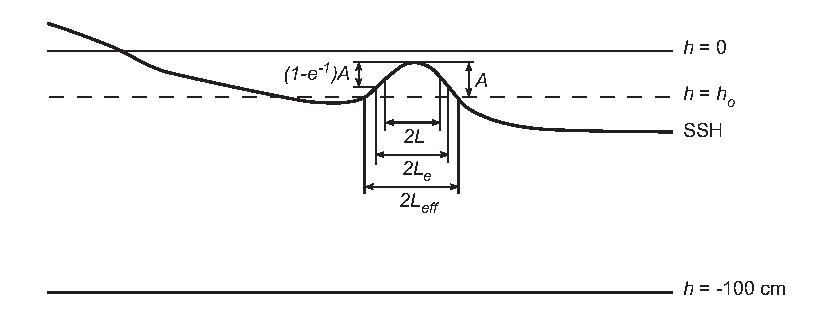
\includegraphics[width=330pt,keepaspectratio=true]{chEs.pdf}
\end{figure}
\end{frame}

\begin{frame}
\frametitle{problematic: broad flat \textit{wobbly} eddies}
 \begin{figure}
\centering
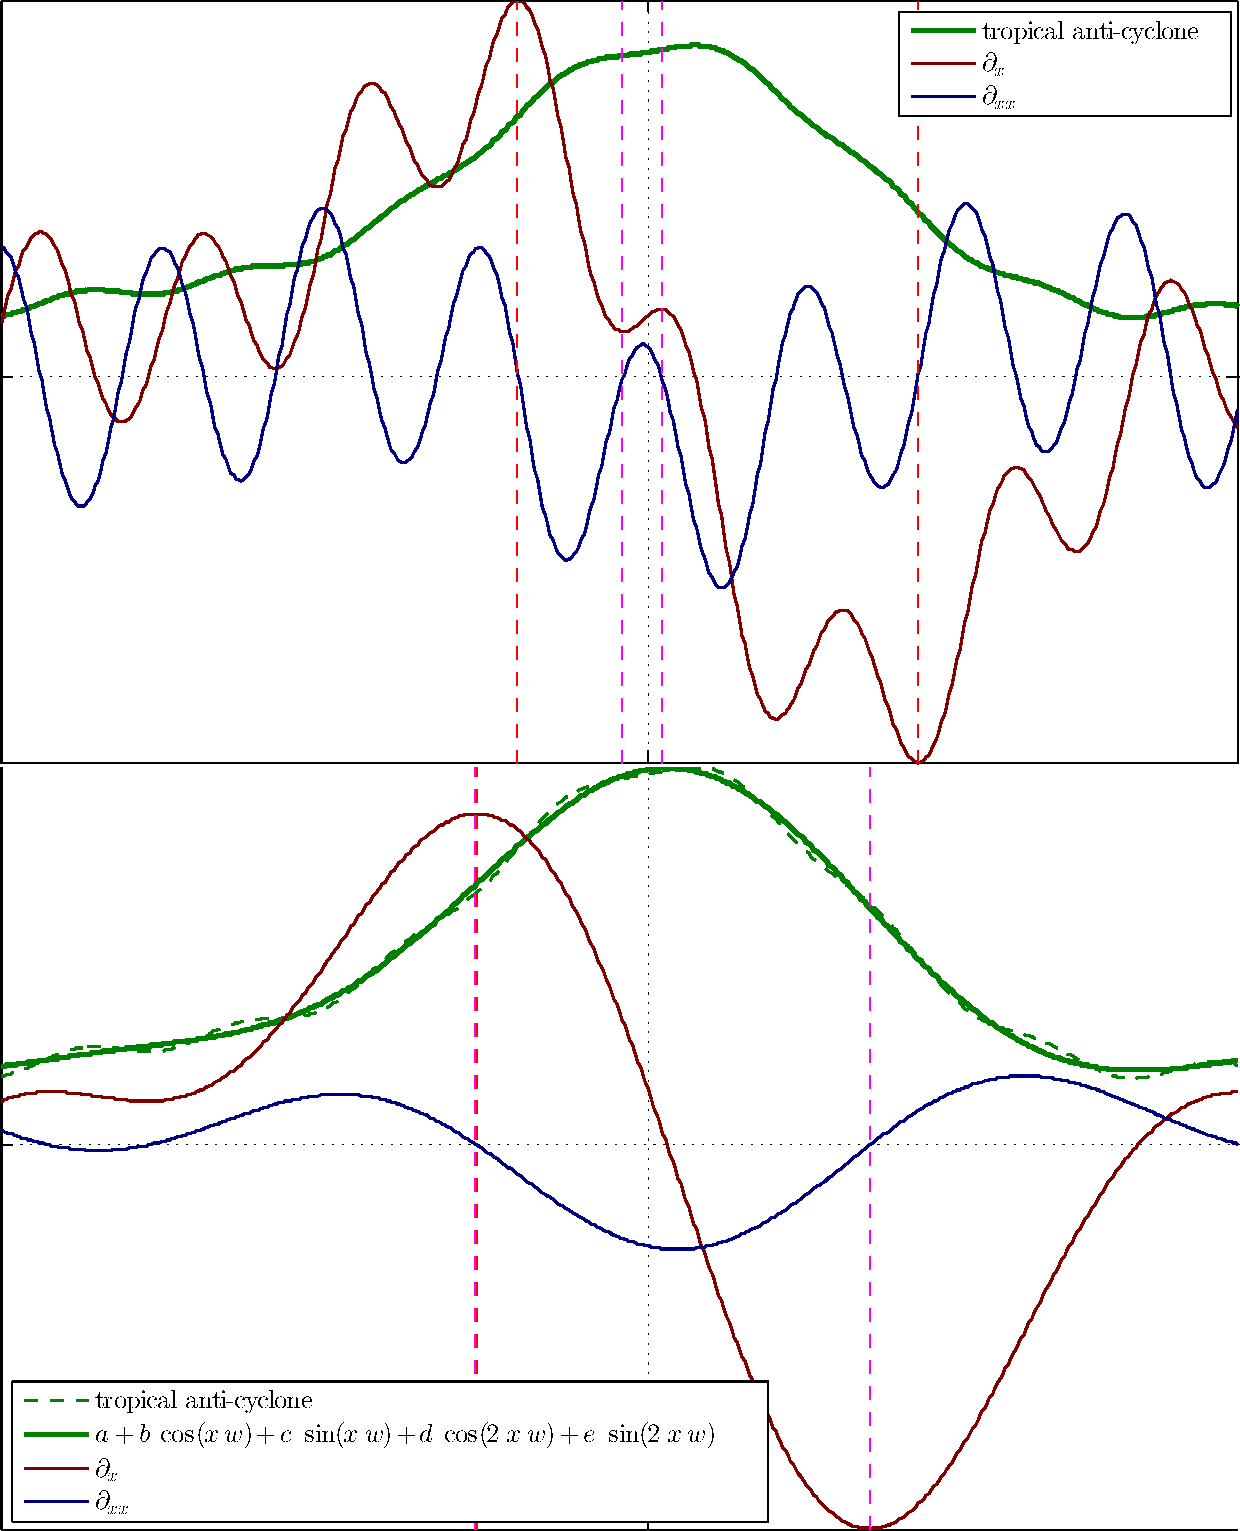
\includegraphics[height=200pt,keepaspectratio=true]{tropicalJmd.pdf}
\end{figure}
\end{frame}

\begin{frame}
	\frametitle{Okubo-Weiss}
	\centering
	\begin{minipage}[T]{1\textwidth}
	\begin{figure}
		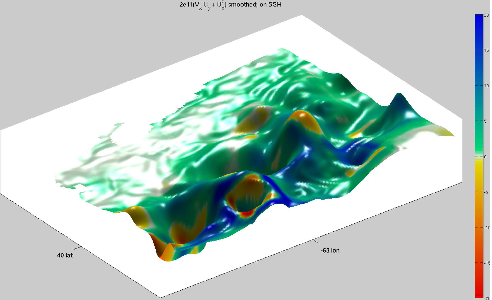
\includegraphics[width=200pt,keepaspectratio=true]{OWpatch2.pdf}
	\end{figure}		
	\end{minipage}
\vfill
	\begin{minipage}[T]{1\textwidth}
		use eigenvalues of 2d deformation tensor to detect vortex: 
		%\begin{align*}
			%%det(\lambda\vec{I} \vec{\Lambda} - \vec{T})=0
			%%&=
			%%(\lambda-u_{x})(\lambda+u_{x}) - v_{x}u_{y} \\
			%%%&=
			%%%\lambda^{2}-u_{x}^{2} - v_{x}u_{y}\\ 
			%\lambda
			%&=
			%\pm \sqrt{u_{x}^{2} + v_{x}u_{y}}
		%\end{align*}
\begin{align*}
& det(\lambda\vec{I}- \vec{\grad \vec{u}}) =0\\
&\lambda^{2} =OW/2=2 u_{x}^{2} + v_{x}u_{y}
\end{align*}	
%\begin{align*}
%& det(\lambda\vec{I}- \vec{\grad \vec{u}}) =0\\
%&\lambda^{2} =OW/2=\tikzmarkin[fill=yellow]{first eq}u_{x}^{2} + v_{x}u_{y}\tikzmarkend{first eq} 
%%&=-(\vort{u})^{2} + (\div{\vec{u}})^{2} + (\grad_{\updownarrow} \cdot \vec{u})^{2}	+ (\underaccent{90^{\circ}}{\grad} \cdot\vec{u})^{2}	\\	&=-vorticity^{2}+divergence^{2}+shear^{2}+stretching^{2}\\& = OW/4
%\end{align*}		
\end{minipage}
\end{frame}


\begin{frame}
\frametitle{Removing larger scale signals important for Chelton's method.}
\begin{figure}
	\centering
	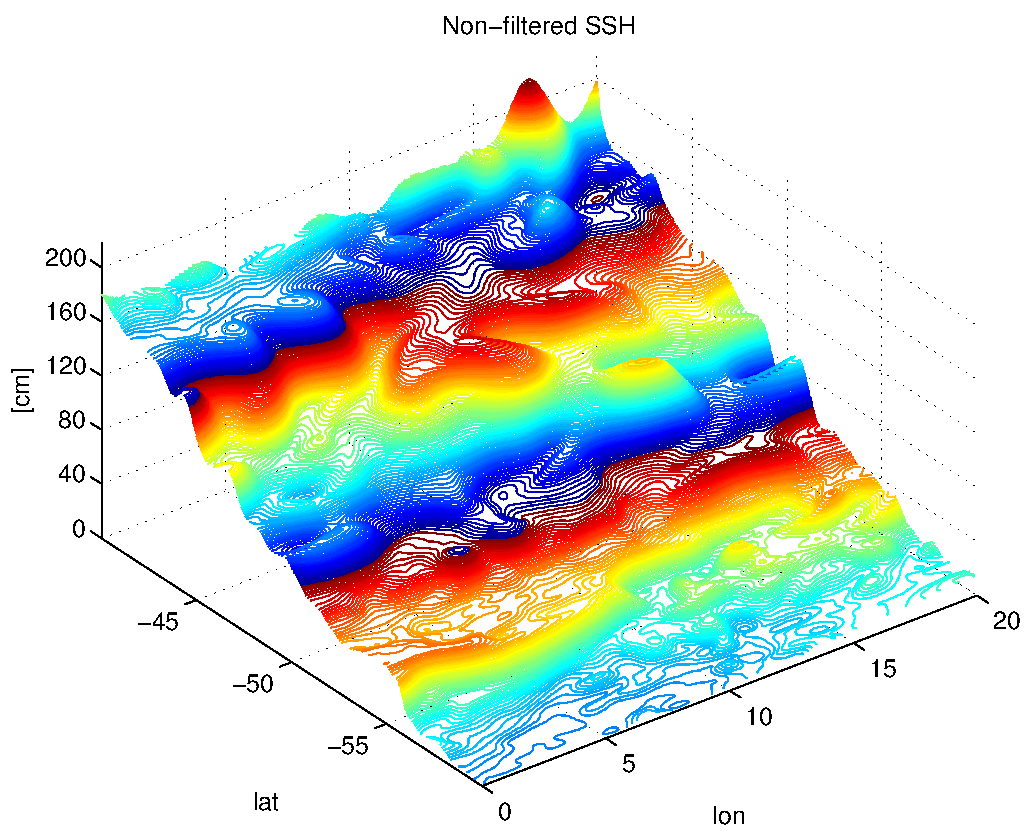
\includegraphics[height=200pt,keepaspectratio=true]{shrunks/Non-filtered_SSH.pdf}
\end{figure}
\end{frame}

\begin{frame}[noframenumbering]
\frametitle{easiest: subtract annual mean}
\begin{figure}
	\centering
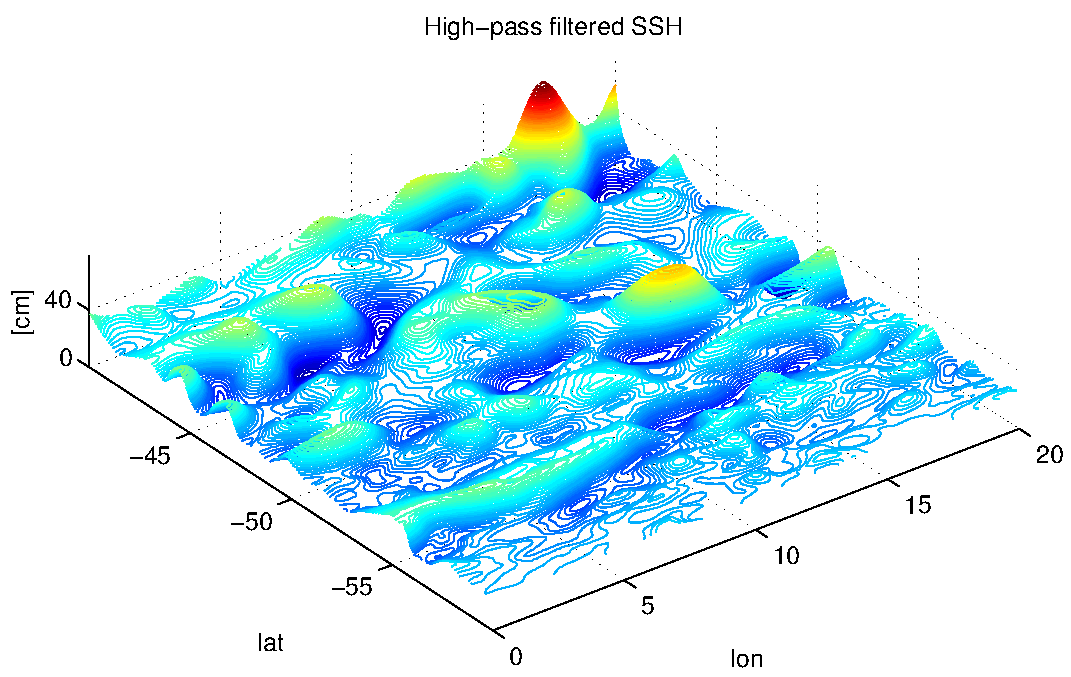
\includegraphics[width=300pt,keepaspectratio=true]{shrunks/High-pass_filtered_SSH.pdf}
\end{figure}
\end{frame}





\begin{frame}
\frametitle{finding a suitable scale threshold}
\begin{figure}
	\centering
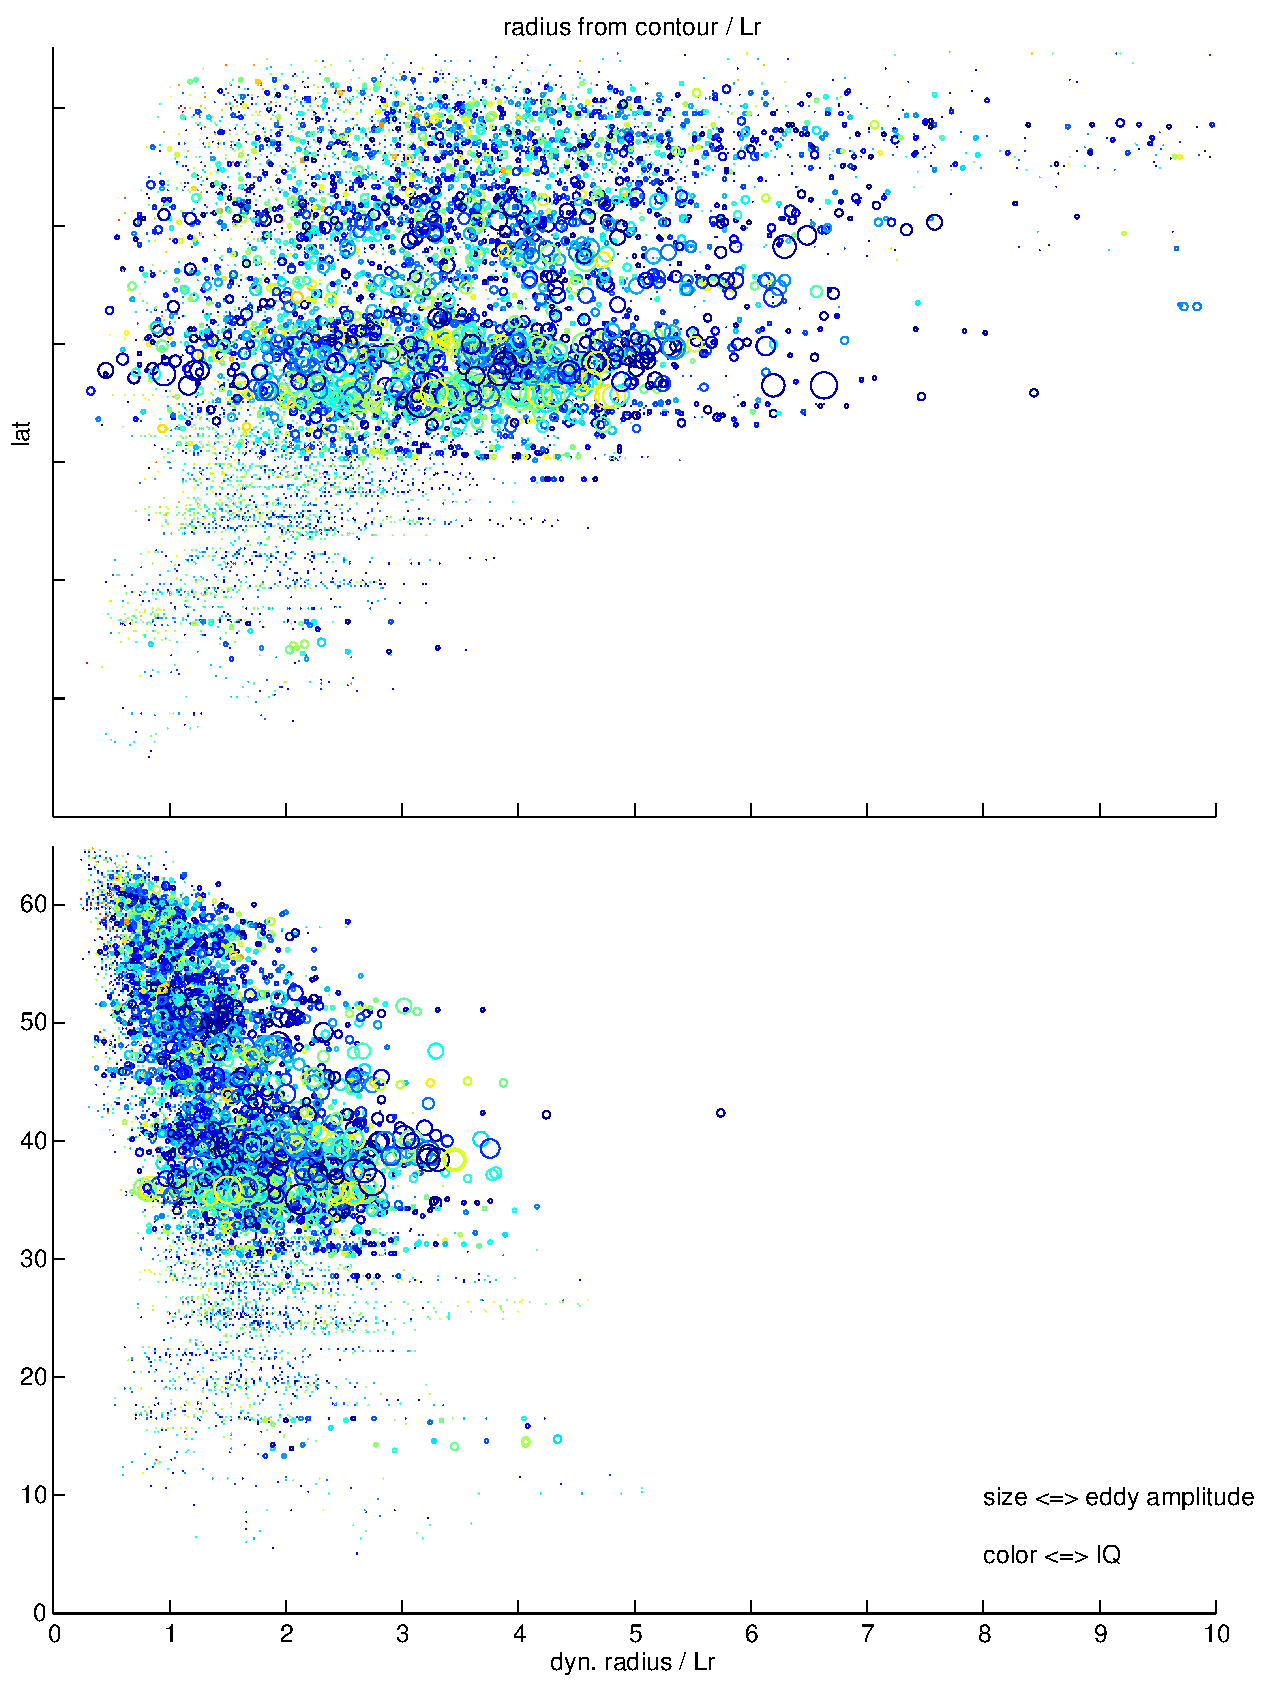
\includegraphics[height=240pt,keepaspectratio=true]{shrunks/scatRadOLrComp.pdf}
\end{figure}
\end{frame}

\begin{frame}[noframenumbering]
\begin{figure}
	\centering
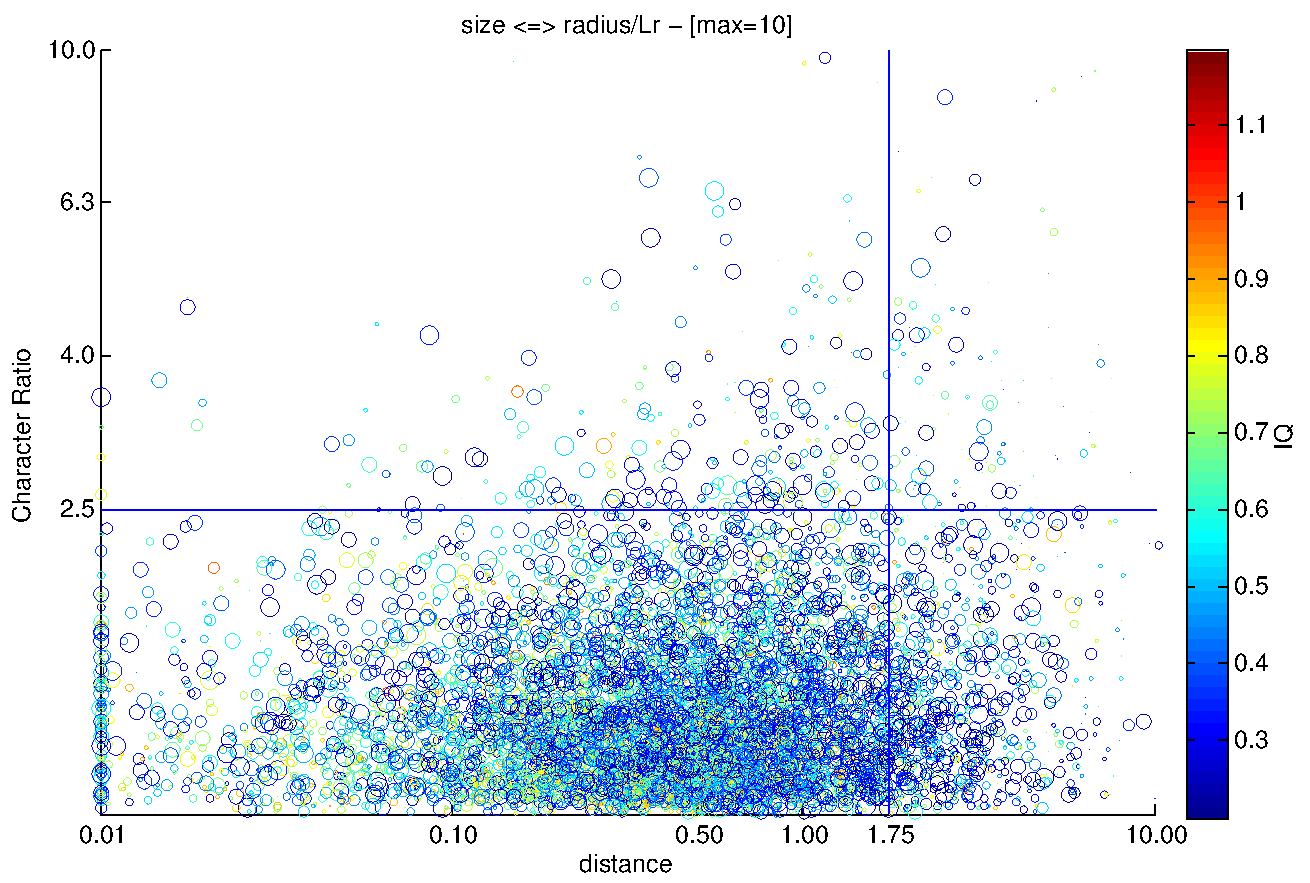
\includegraphics[width=300pt,keepaspectratio=true]{shrunks/scat1.pdf}
\end{figure}
\end{frame}

\begin{frame}[noframenumbering]
\begin{figure}
	\centering
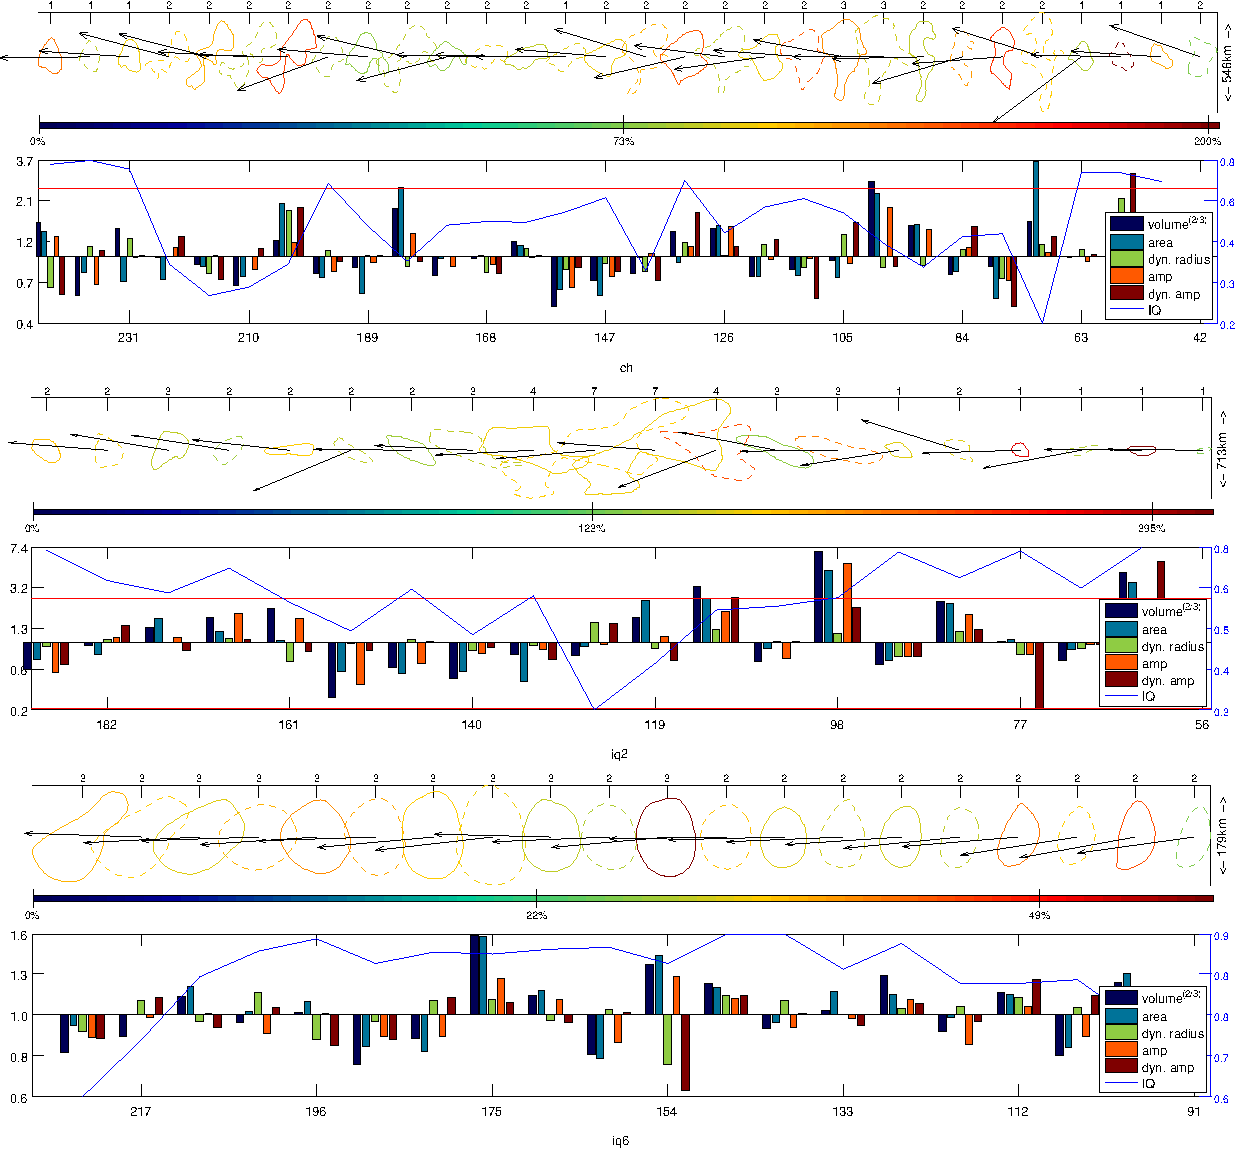
\includegraphics[height=260pt,keepaspectratio=true]{parAnalAll.pdf}
\end{figure}
\end{frame}


\begin{frame}[noframenumbering]
\begin{figure}
	\centering
	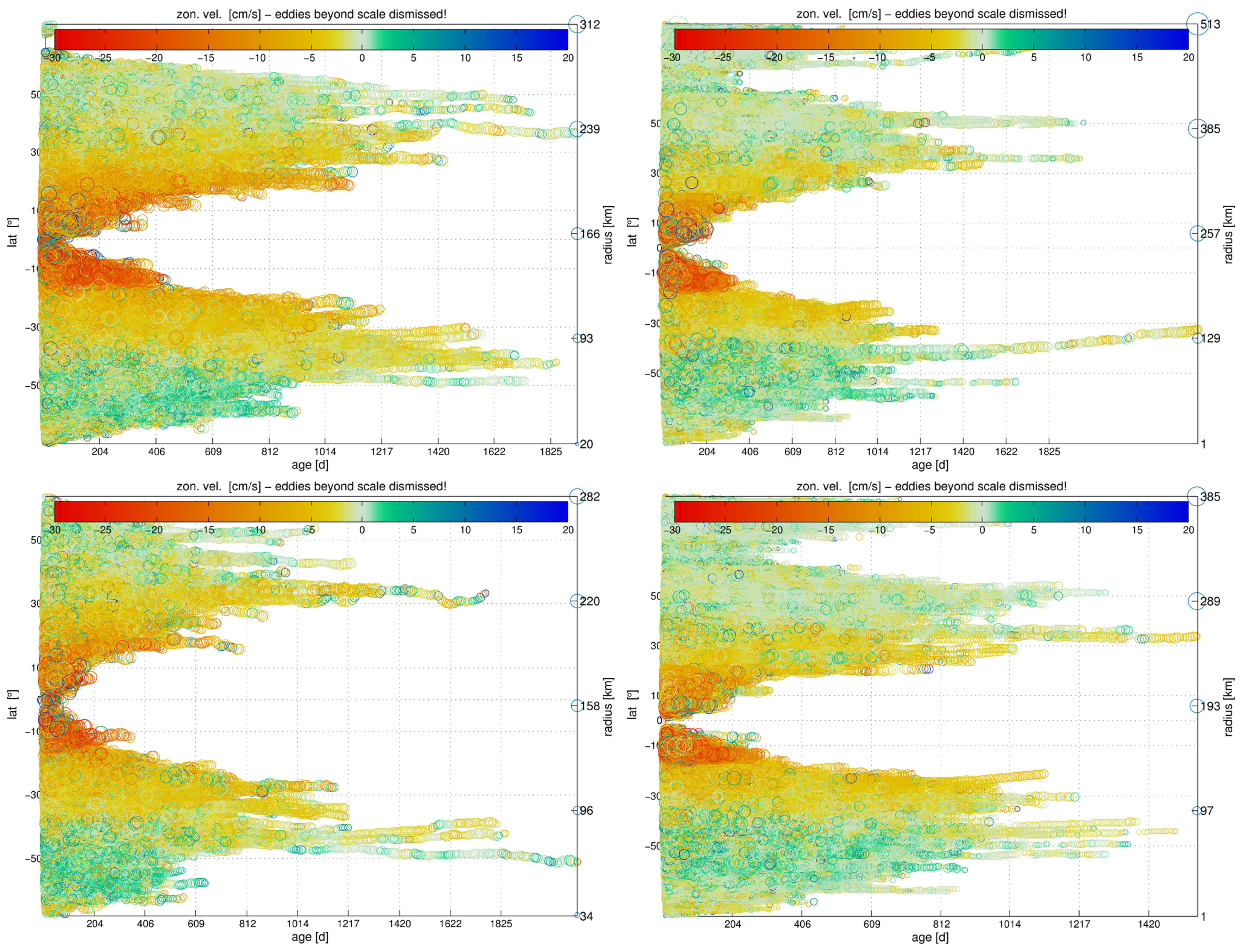
\includegraphics[width=300pt,keepaspectratio=true]{SCTall.pdf}
\end{figure}
\end{frame}


%% appendix



%\begin{frame}
%\frametitle{assume gauss shape:  $A \exp{\left(- x^2/2\sigma^2\right)}$}
 %\begin{figure}
%\centering
%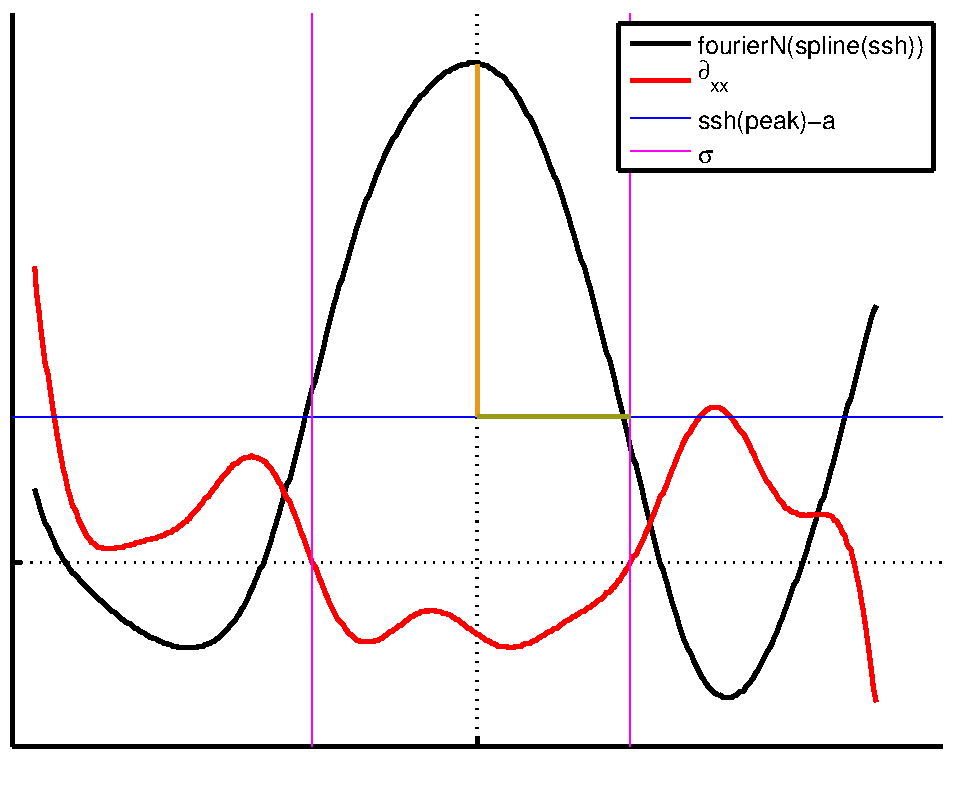
\includegraphics[height=200pt,keepaspectratio=true]{Ne.pdf}
%\end{figure}
%\end{frame}



%\begin{frame}	
%\begin{align*}
	%\left| \lambda \vec{I} - \grad \vec{u} \right|
	%&=
%\begin{vmatrix}
 %\lambda - u_{x} & u_{y} \\
 %v_{x} & \lambda - v_{y}
 %\end{vmatrix}	\\
 %&=
 %\left(  	\lambda - u_{x} \right)  \left( 	\lambda - v_{y} \right){}
 %- v_{x} u_{y}\\
 %\lambda^{2}&=
 	  %u_{x}^{2}
 %+ v_{x} u_{y}
%\end{align*}

%\begin{align*}
	%\left| \lambda \vec{I} - \vec{\Omega}  \right|
	%&=
%\frac{1}{2}\begin{vmatrix}
 %\lambda & u_{y}-v_{x} \\
 %-u_{y}+v_{x} & \lambda 
 %\end{vmatrix}	\\
 %2\lambda_{\Omega}^{2}
 %&=
 %u_{y}^{2}-2u_{y}v_{x}+v_{x}^{2}
%\end{align*}

%\begin{align*}
	%\left| \lambda \vec{I} - \vec{E}  \right|
	%&=
%\frac{1}{2}\begin{vmatrix}
 %\lambda -2u_{x} & u_{y}+v_{x} \\
 %u_{y}+v_{x} & \lambda -2v_{y}
 %\end{vmatrix}	\\
 %%&(\lambda -2u_{x} ) (\lambda +2u_{x})
 %%-u_{y}^{2}-2u_{y}v_{x}-v_{x}^{2}  
 %%\\
  %2\lambda_{E}^{2}
 %&=4u_{x}^{2}
 %+u_{y}^{2}
 %+ 2u_{y}v_{x}
 %+v_{x}^{2}  
%\end{align*}
%\begin{align*}
	%-\lambda_{\Omega}^{2} + \lambda_{E}^{2}
	%&=
	 %2u_{y}v_{x}
	 %+2u_{x}^{2}
%\end{align*}



%\end{frame}



%\begin{frame}
%\begin{align*}
%&=-(v_{x}-u_{y})^{2}
%+(u_{x}+v_{y})^{2}
%+(v_{x}+u_{y})^{2}
%+(u_{x}-v_{y})^{2}\\
%&=
%-(
%v_{x}^{2}
%-2v_{x}u_{y}
%+u_{y}^{2}
%)
%+0+
%(
%v_{x}^{2}
%+2v_{x}u_{y}
%+u_{y}^{2}
%)
%+(
%u_{x}^{2}
%-2u_{x}v_{y}
%+v_{y}^{2}
%)\\
%&=
%4v_{x}u_{y}
%+(
%u_{x}^{2}
%-2u_{x}v_{y}
%+v_{y}^{2}
%)\\
%&=
%4v_{x}u_{y}
%+
%4u_{x}^{2}
%\\
%\end{align*} 
%\end{frame}










